% AUTHOR: Diego Sarceno
% Last Update: 11.07.2020

\documentclass[11pt, spanish, letterpaper]{article} %tipo de documento

\usepackage[letterpaper]{geometry} %margenes
\geometry{verbose,tmargin=2.5cm,bmargin=2.5cm,lmargin=2cm,rmargin=2cm}
\usepackage{amsmath,amsthm,amssymb} %modos matemáticos y  simbolos
\usepackage{latexsym,amsfonts} %simbolos matematicos
\usepackage{cancel} %hacer la linea que cancela las ecuaciones
\usepackage[spanish, es-noshorthands]{babel} %comandos en español y cambia el cuadro por la tabla
\decimalpoint %cambia las comas por puntos decimal
\usepackage[utf8]{inputenc} %caracteristicas del español
\usepackage{physics} %Simbolos fisicos
\usepackage{array} %mejores formatos de tabla
\parindent =0cm %sangria
\usepackage{graphicx} %graficas e imagenes
\usepackage{mathtools}
\usepackage[framemethod=TikZ]{mdframed}%Entornos talegas
\usepackage[bookmarksnumbered,
			colorlinks = true,
			linkcolor = blue,
			citecolor = black,
			urlcolor = black]{hyperref}%formato de los links y URL's
\usepackage{multicol} %varias columnas
\usepackage{enumerate} %enumeraciones
\usepackage{pgf,tikz,pgfplots} %documentos en formato tikz
\usepackage{mathrsfs} %letras chingonas (transformada de laplace)
\usepackage{subfigure} %varias figuras seguidas
%\usepackage[square,numbers]{natbib} %bibliografias
%\usepackage[nottoc]{tocbibind}
%\bibliographystyle{plainnat}
\usetikzlibrary{arrows, babel, calc}
\usepackage{tabulary}
\usepackage{multirow} %ocupar varias filas en una tabla
\usepackage{fancybox} %recuadros talegas
\usepackage{float} %ubicar graficas
\usepackage{color}
\usepackage{comment}
\usepackage{stackrel}
\usepackage{calligra}
\usepackage{lipsum} % texto de relleno
\usepackage{cite}
\usepackage{circuitikz} % crear circuitos
\usepackage{listings} % permite el ingreso de codigo
%\usepackage{showframe}
%\usepackage{LobsterTwo}
% NEW PACKAGES
\usepackage{makeidx}
\usepackage{authblk} % para la manipulación de autores y afiliación
\usepackage{booktabs}
\usepackage{colortbl}
\usepackage{bbold}
\usepackage{dsfont}
\usepackage{tensor}
\usepackage{colortbl}
\usepackage{amsbsy}
\usepackage[draft,inline,nomargin]{fixme} \fxsetup{theme=color}

%This defines my comments
\definecolor{mycolor}{RGB}{250,0,0}
\FXRegisterAuthor{ds}{sds}{\color{mycolor}DS}





%%%%%%%%%%%%%%%%%%%%%%%%%%%%%%%%%%%%%%%%%%%%%%%%%%%%%%%%%%%
\lstset{basicstyle=\ttfamily,breaklines=true}
\lstset{numbers=left, numberstyle=\tiny, stepnumber=1, numbersep=6pt}
\lstset{emph={import,as,return,for,in,else,if,def,True,False,append}, emphstyle=\color{blue}, emph={[2]pKronecker},
emphstyle={[2]\color{violet}}, emph={[3]float,input,int,range,print,len},
emphstyle={[3]\color{violet}}}
\lstset{morecomment=[l][\color{gray!40}]{\#}, morestring=[b][\color{green!50!black}]"}
%%	Importe de archivo: \lstinputlisting[inputencoding=latin1]{'nombre del archivo'.py}
%%%%%%%%%%%%%%%%%%%%%%%%%%%%%%%%%%%%%%%%%%%%%%%%%%%%%%%%%%%
\setlength{\columnseprule}{0pt}
%-------------------------------------------------
\newcommand{\N}{\mathbb{N}}
\newcommand{\Z}{\mathbb{Z}}
\newcommand{\Q}{\mathbb{Q}}
\newcommand{\I}{\mathbb{I}}
\newcommand{\R}{\mathbb{R}}
\newcommand{\C}{\mathbb{C}} %Conjuntos numericos
\newcommand{\F}{\mathbb{F}} %Campo Cualquiera
\newcommand{\Pos}{\mathbb{P}} %Reales positivos
\newcommand{\f}{\textit{f}} %f de funcion
\newcommand{\g}{\textit{g}}
\newcommand{\kernel}{\mathscr{N}} %kernel
\newcommand{\range}{\mathcal{R}} %range
\newcommand{\lagran}{\mathcal{L}} %lagrangiano
\newcommand{\laplace}{\mathscr{L}} %transformada de laplace, mapas lineales
\newcommand{\M}{\mathcal{M}} %Matrices
\newcolumntype{E}{>{$}c<{$}} %entorno matematico en columnas de una tabla
\newcommand{\vi}{\boldsymbol{\hat{\imath}}}
\newcommand{\vj}{\boldsymbol{\hat{\jmath}}}
\newcommand{\vk}{\vu{k}}%vectores unitarios R3
\newcommand{\vr}{\hat{r}}
\newcommand{\vp}{\boldsymbol{\hat{\phi}}}
\newcommand{\vz}{\vu{z}}%vectores unitarios en cilindricas
\newcommand{\vaz}{\boldsymbol{\hat{\theta}}}%vectores unitarios en esféricas
\newcommand{\vx}{\vu{x}}%vectores
\newcommand{\vy}{\vu{y}}%vectores 
\newcommand\numberthis{\addtocounter{equation}{1}\tag{\theequation}}
\newcommand{\LI}{\lim _{h\longrightarrow 0}}
\newcommand{\SU}{\longrightarrow \sum _{n=0} ^{\infty}}
\newcommand{\QED}{\hfill {\qed}}
\newcommand{\cis}{\text{cis} \,}
%----------------------------------------------------------
%----------------------------------------------------------


%-paquete para unidades en el sistema internacional
\usepackage[load=prefix, load=abbr, load=physical]{siunitx}
\newunit{\gram}{g }%gramos
\newunit{\velocity}{ \metre / \Sec }%unidades de velocidad sistema internacional
\newunit{\acceleration}{ \metre / \Sec^2 }%unidades de aceleracion sistema internacional
\newunit{\entropy}{ \joule / \kelvin }%unidades de entropia sistema internacional
%--definiendo constantes fisicas en el SI
\newcommand{\accgravity}{9.8 \metre / \Sec^2}
%---diferencial inexacta
\newcommand{\dbar}{\mathchar'26\mkern-12mu d}
%-------------------------END-------------------------------------
%------------------------Barra negra-------------------------------
\tikzset{
	warningsymbol/.style={
		rectangle,draw=black,
		fill=white,scale=1,
		overlay}}
\mdfdefinestyle{warning}{%
	hidealllines=true,leftline=true,
	skipabove=12,skipbelow=12pt,
	innertopmargin=0.4em,%
	innerbottommargin=0.4em,%
	innerrightmargin=0.7em,%
	rightmargin=0.7em,%
	innerleftmargin=1.7em,%
	leftmargin=0.7em,%
	middlelinewidth=.2em,%
	linecolor=black,%
	fontcolor=black,%
	firstextra={\path let \p1=(P), \p2=(O) in ($(\x2,0)+0.5*(0,\y1)$)
										node[warningsymbol] {$\mathcal{S}$};},%
	secondextra={\path let \p1=(P), \p2=(O) in ($(\x2,0)+0.5*(0,\y1)$)
										node[warningsymbol] {$\mathcal{S}$};},%
	middleextra={\path let \p1=(P), \p2=(O) in ($(\x2,0)+0.5*(0,\y1)$)
										node[warningsymbol] {$\mathcal{S}$};},%
	singleextra={\path let \p1=(P), \p2=(O) in ($(\x2,0)+0.5*(0,\y1)$)
										node[warningsymbol] {$\mathcal{S}$};},%
}
%%%%%%%%%%%%%%%%%%%%%%%%%%%%%%%%%%% Tema - BEGIN
\newtheoremstyle{Tema}% name of the style to be used
  {0mm}% measure of space to leave above the theorem. E.g.: 3pt
  {10mm}% measure of space to leave below the theorem. E.g.: 3pt
  {}% name of font to use in the body of the theorem
  {}% measure of space to indent
  {\bfseries}% name of head font
  {\newline}% punctuation between head and body
  {30mm}% space after theorem head
  {}% Manually specify head

\theoremstyle{Tema} \newtheorem{Tema}{Tema} %%%%% Template para Temas
\theoremstyle{Tema} \newtheorem{serie}{Serie}              %%%%%  Template para Series de ejercicios
\theoremstyle{Tema} \newtheorem{teorema}{Teorema}              %%%%%  Template para Teoremas
\theoremstyle{Tema} \newtheorem{pregunta}{Pregunta}              %%%%%  Template para Series de ejercicios
\theoremstyle{Tema} \newtheorem{ejercicio}{Ejercicio}    %%%%%  Template para Ejercicios
\theoremstyle{Tema} \newtheorem{ejemplo}{Ejemplo}    %%%%%  Template para Ejemplos
\theoremstyle{Tema} \newtheorem{solucion}{Solución}    %%%%%  Template para Soluciones
\theoremstyle{Tema} \newtheorem{problem}{Problema}    %%%%%  Template para Problema
\theoremstyle{Tema} \newtheorem{definicion}{Definición}    %%%%%  Template para Soluciones
\theoremstyle{Tema} \newtheorem{proposicion}{Proposición}    %%%%%  Template para Soluciones
\theoremstyle{Tema} \newtheorem{lema}{Lema}    %%%%%  Template para Soluciones
%-------------------------END-------------------------------------


% COMPILAR USANDO

% pdflatex template
% bibtex template
% pdflatex template
% pdflatex template




% para los metadatos del PDF
%\usepackage[%
%bookmarksnumbered,%
%pdfauthor={Diego Sarceño (dsarceno68@gmail.com)},%
%pdftitle={Puntos de Lagrange},%
%pdfsubject={Proyecto},%
%pdfkeywords={template, template}]{hyperref}

\title{\sc Problema de los 3 Cuerpos, Puntos de Lagrange}%
\author{Diego Sarceño \thanks{Escuela de Ciencias Físicas y Matemáticas,
  Universidad de San Carlos de Guatemala.}}
\date{Guatemala, \today}
%% 20210307

\begin{document}  
\maketitle

\begin{abstract}
  \lipsum[1]
\end{abstract}


\section{Introducción}
\label{sec:intro}
\justify 
\lipsum[1]
% 
\begin{displaymath}
  \int_a^b f(x) dx,
\end{displaymath}
%
\lipsum[1]

\section{Puntos de Lagrange}
\subsection{Problema de los Tres Cuerpos}
\label{sec:Puntos de Lagrange}

El problema de los tres cuerpos no es soluble analíticamente; sin embargo, realizando ciertas restricciónes al problema llega a poderse resolver. Consideraciones a tomar:
\begin{enumerate}
	\item Dos cuerpos masivos en orbitas circulares alrededor de su centro de masa.
	\item El tercer objeto de masa $m$ tiene la condición: $m\ll M_1,M_2$, donde $M_1$ y $M_2$ son las masas de los dos objetos anteriormente mencionados.
\end{enumerate}

\subsubsection{Problema de los dos Cuerpos}
Partiendo del problema conocido de los dos cuerpos, el cual ya es conocido, se toma el sistema respecto de un punto de referencia $O$

\begin{figure}[H]
  	\centering
  	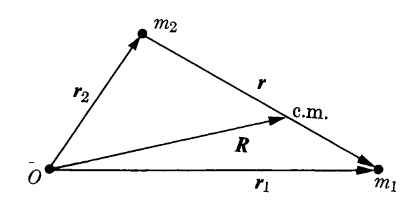
\includegraphics[scale=0.5]{Images/twoBodyProblem.png}
  	\caption{Posición de ambos cuerpos en el espacio, representando su posicion relativa y respecto a un sistema de coordenadas $O$. El vector $\vb{R}$ representa la posición del centro de masa relativa al sistema $O$. Imagen extraída de \cite{b1}, cap $4$.}
  	\label{fig:twoBodyProblem}
\end{figure}

Además, la ecuación de movimiento
\begin{displaymath}
	\mu \ddot{\vb{r}_{21}} = \vb{F}, \quad \quad \mu = \frac{M_1 M_2}{M_1 M_2},
\end{displaymath}

\noindent
al término $\mu$ se le conoce como masa reducida\footnote{De \cite{b2} capítulo $8$, sección $2$}. Para la fuerza gravitacional y una trayectoria circular, la expresión para frecuencia angular del sistema, se tiene
\begin{displaymath}
	\omega ^2 = \frac{G(M_1 + M_2)}{a^3}.
\end{displaymath}
 
\subsubsection{Sistema de Referencia Estrellado}

Para simplificar el análisis del problema, se introduce un sistema en movimiento, en concreto, en rotación. Esto es para eliminar el movimento de los cuerpos más masivos, a este nuevo sistema le llamaremos $O^*$. Este nuevo sistema tendrá su origen en el centro de masa y, a la distancia entre los cuerpos se le llamará $a$. De modo que las posiciónes en $O^*$ están dadas solo en el eje $x^*$ como
\begin{displaymath}
	x_1 = \frac{M_2}{M_1 + M_2}, \quad x_2 = -\frac{M_1}{M_1 + M_2};
\end{displaymath}

\noindent
además, se fija $\vec{\omega} = \omega \vz$ y la masa $m$ solo se mueve en el plano $x^* y^*$. Con todo esto, la ecuación de moviento en el sistema $O^*$
\begin{displaymath}
	m\frac{\text{d}^{*2} r}{\text{d} t^2} = F_1 + F_2 - m\omega \cp (\omega \cp r) - 2m\omega \cp \frac{\text{d}^* r}{\text{d} t}.
\end{displaymath}

\noindent
En la cual las dos fuerzas representadas son las fuerzas de cada una de las masas sobre la masa $m$ orbitando. Expresandolas en componentes
\begin{displaymath}
	F_1 = \frac{GM_1 m}{\qty((x - x_1)^2 + y^2)^{\flatfrac{3}{2}}} (x - x_1,y), \quad \quad F_2 = \frac{GM_2 m}{\qty((x - x_2)^2 + y^2)^{\flatfrac{3}{2}}} (x - x_2,y).
\end{displaymath}


Analizando el resto de términos, se tiene que la fuerza de coriolis es perpendicular a la velocidad, por lo que no tiene un potencial asociado. Para el término de la fuerza centrífuga, es sencillo corroborar que es una fuerza central\footnote{Fuerza radial conservativa.}, lo que implica que tiene una energía potencial asociada. Desarrollando el término de la fuerza centrífuga y encontrando el potencial
\begin{align*}
	- m\omega \cp (\omega \cp r) &= m\omega ^2 \qty(x\mathbb{\vu{x} ^*} + y \mathbb{\vu{y} ^*}) \\
	V_c &= -\frac{1}{2} m\omega ^2 (x^2 + y^2).
\end{align*}

Con el análisis anterior, se concluye que la enería potencial total del sistema es
\begin{displaymath}
	V = -\frac{GM_1 m}{\qty((x - x_1)^2 + y^2)^{\flatfrac{1}{2}}} - \frac{GM_2 m}{\qty((x - x_2)^2 + y^2)^{\flatfrac{1}{2}}} - \frac{1}{2} m\omega ^2 \qty(x^2 + y^2).
\end{displaymath}

\noindent
Por simplicidad no se tomara la enería potencial, sino que el potencial gravitacional del sistema, por simplicidad al momento de desarrollar los calculos
\begin{displaymath}
	\mathcal{G} = -\frac{GM_1}{\qty((x - x_1)^2 + y^2)^{\flatfrac{1}{2}}} - \frac{GM_2}{\qty((x - x_2)^2 + y^2)^{\flatfrac{1}{2}}} - \frac{1}{2} \omega ^2 \qty(x^2 + y^2).
\end{displaymath}


\subsection{Puntos de Lagrange}
Para un sistema de dos cuerpos, los puntos de lagrange son las posiciones en donde un objeto/satélite podría estar en reposo respecto al sistema orbital. Estos puntos representan las posiciones en donde la atracción del sistema presenta una rotación sincrónica con la menor masa del sistema. Matemáticamente hablando, son las soluciones de equilibrio al problema de los $3$ cuerpos restringido. Para cualquier sistema de $3$ cuerpos existen $5$ de estos puntos de lagrange, representados por $L_1,L_2,L_3,L_4$ y $L_5$. 


\section{Resultados}
\label{sec:resultados}
\lipsum[1-2]

\begin{figure}[H]
  \centering
  %\includegraphics[width=.85\textwidth]{images/TrapSerr}  
  \caption{Error relativo de la aproximación en función del número de
    trapecios. Fuente: elaboración propia.}
  \label{fig:Serror}
\end{figure}

\lipsum[1-2]



\section{Conclusiones}
\label{sec:conclusiones}

\lipsum[1-2]

\begin{figure}[H]
  \centering
  % \includegraphics[width=.85\textwidth]{images/TrapMerr}  
  \caption{Área bajo la curva obtenido medidante las dos implementaciones,
    secuencial y paralelo en función del número de trapecios.  En el inserto
    está la diferencia del valor obtenido en la implementación secuencial
    menos el valor obtenido en la implementación paralela.  Fuente:
    elaboración propia.}
  \label{fig:Merror}
\end{figure}


\lipsum[1-2]

\section*{Agradecimientos}
\label{sec:agradecimientos}

Se agradece a la ECFM-USAC por el uso del clúster Euclides donde se realizaron
las pruebas de rendimiento reportadas en este trabajo.

% References
\nocite{*}
\bibliographystyle{IEEEannot}%
\bibliography{references}%

\begin{thebibliography}{00}
\bibitem{b1} R. Symon, \textit{Mechanics} 3a. Ed. Addison$-$Wesley Publishing Company, 1971
\bibitem{b2} R. Taylor, \textit{Classical Mechanics}, Edwards Brothers, Inc. 2005.
\end{thebibliography}

\end{document}




%%% Local Variables:
%%% mode: latex
%%% TeX-master: t
%%% End:
